\section{The Aggregator}\label{aggregator}
As mentioned in Chapter~\ref{github}, I decided to use Github as my data source and to utilize their \emph{Github APIv3} for this purpose.
This \ac{api} is publicly available and can be used by anyone registered on Github.
In this chapter I will explain the technologies and methods used in the data aggregation process, the database structure and show some problem which occurred during the duration of this thesis.


\subsection{Gitalizer's Database}\label{data-structure}
To store the gathered Information I chose a \ac{sql} based solution.
PostgreSQL provides excellent tools to provide a high consistency in your database, namely check constraints, as well as great support for working with times, time zones and locations.

The usage of a \ac{sql} database in the combination with an \ac{orm} allows to write highly specific queries and provides some other convenient features I will cover later in this section.

\subsubsection{Database Design}
The schema created for the purpose of this thesis consists of five \ac{orm} models.
There is a model for Commits, Emails and Repositorys, Contributers as well as Organizations.
The latter is only important to validate results and is not actually used for knowledge discovery, as this is Github specific data.

\begin{figure}[H]
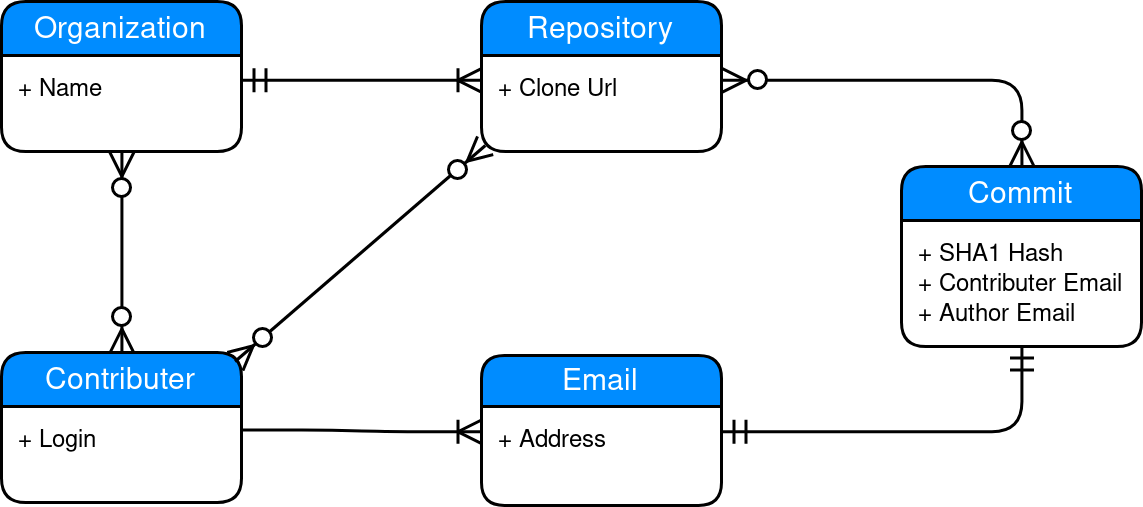
\includegraphics[scale=0.27]{./graphs/gitalizer-data-structure}
\centering
\caption{Gitalizer database relationships.}\label{fig:gitalizer-relationship}
\end{figure}

Every commit of each repository is saved in the database along with its \ac{sha1} hash and the two email addresses as in listing~\ref{lst:raw-commit}.
It is important to note that there is a many-to-many relationship in figure~\ref{fig:gitalizer-relationship} between commits and repositories.
This feature prevents duplication of the same commits from forked repositories.
It is for instance a common practice to create a fork of a repository to develop without intervening with the main git repository of the project.
As described in Section~\ref{internal representation} the probability of a \ac{sha1} collision is extremely low.
By exploiting this feature it is possible to enforce a unique constraint on the commit hash column, assuming that any duplicated commit hash actually results from a forked or copied repository.
Without this mechanism it could be possible that the same commit of a contributer could be used multiple times as a result of repository forking.
After collecting 43 million commits from Github and actively ignoring obvious project forks, there are still 49 million references between commits and repositories.
This means that about 13\% of gathered commits result from forked repositories which can not easily identified as such.

As stated above each commit is also saved with its respective email addresses.
There exists a one-to-many relationship between contributers and emails, as every contributer can obtain an unlimited amount of email addresses.
To unambiguously assign a commit to a person, it is necessary to connect all commits email addresses to this person.
This relationship does not have a \inlinecode{NOT NULL} constraint as it happens quite often that an email address can not be assigned to any person.
Looking at the collected data it appears that roughly 20\% of collected email addresses from Github are no longer connected to an active user.

The last model of the database schema is the organization.
As stated in section~\ref{github-organization} Github provides a way to organize several people in organizations and teams.
As one of the goals of this thesis is to see if it is possible to detect member of an organization in open-source projects, this data can be used to check against the results of this research's results.


\subsection{Gitalizer}
The program I wrote for this thesis is named Gitalizer and features data aggregation, preprocessing, knowledge extraction and visualization.
Gitalizer uses a PostgreSQL database for data storage and data consistency checks as described in~\ref{data-structure}.
For interaction with the Github \ac{api} the \emph{PyGithub} library is used, which provides a convenient abstraction layer for requests and automatically maps \ac{json} responses to python objects.


\subsubsection{Methods}
The data aggregation module of Gitalizer is capable of several scanning methods.
In the following we will look at these approaches in detail.

\subsubsection{Stand-alone Repository}\label{stand-alone-repository-scan}
Gitalizer can scan any git repository from a \ac{ssh} or \ac{http} \acs{url} as long as it has access to it.
At first the repository is cloned into a local directory.
When the cloning is done the scan process begins.
During the scan, we checkout the \emph{HEAD} of the current default branch for this repository and walk down every commit of the Git history.
The program saves all available meta data for each commit in its database, namely the emails, timestamps and names of the committer as well as additions and deletions to the project in lines of code.

After this scan we are still missing a lot of information.
The unique identifier of an author or committer is their email address, as names may change or can be ambiguous.
The problem with the simplicity of Git is that there doesn't exist the concept of an user.
Thereby we cannot easily link email addresses to a specific contributer.


\subsubsection{Github Repository}\label{github-repo-scan}
To tackle the problems in~\ref{stand-alone-repository-scan}, I used the Github \ac{api} to get some of the missing meta data.
The general approach is the same as in the previous scan method. The repository is cloned and locally scanned.
However, a request to Github is issued every time a new email is found that we do not already have linked to a contributer.
Github allows to link multiple email addresses with a single user account and automatically references the respective user in their own \ac{api} commit representation.
With this additional meta data we gain ground truth about the identity of an author or committer.

Anyway this approach does not work, if the user of a commit removed the email used for the commit from his account, or if the user deleted his account.
In this case there is nothing that can be done and these commits need to be handled later on in the preprocessing of the data.


\subsubsection{Github User}\label{github-user-scan}
To get all repositories of a specific user, I implemented a new functionality utilizing the Github \ac{api}.
At first several requests are issued to get all repositories of the specified user, as well as all starred repositories of this user.
For each starred repository we check if the user contributed to this repository, which is quite easy as the \ac{api} provides an endpoint for this query.
During the repository exploration, every relevant repository is added to a shared queue, lets call it ``repo-queue'', which is then processed by a multiprocessing pool of workers.
Each worker process scans a single repository as described in~\ref{github-repo-scan}.


\subsubsection{Github connected User}\label{github-user-remote-scan}
For detection and analysis of connections between contributers over multiple repositories, I needed to gather as many repositories of related users as possible.
Gitalizer is able to achieve this by not just scanning a single user, but rather scanning the repositories of the specific user, as well as the repositories of all following and followed users.
For this task two different worker pools are utilized.
The user pool is initialized with a shared queue, lets call it ``user-queue'', of all users we need to look at.
This pool simply searches for relevant repositories of a single user and passes them to a second shared queue.
The second pool then processes the ``repo-queue'' as described in~\ref{github-repo-scan}.

For organizations it's nearly the same approach.
Initially all repositories, which are owned by the organization, are added to the ``repo-queue''.
All publicly visible organization members are then added to the ``user-queue'' and processed as described above.


\subsection{Problems}
During the development of the data aggregator I experienced a few problems and edge cases which needed to be handled.
The earliest and most delaying problem was the rate limit of the Github \ac{api}.
The first version of the aggregator didn't clone and scan the repository locally, but rather gathered all information from the Github \ac{api} endpoints.
This approach worked well until the aggregator hit the official repository of Nmap, which has about 11.000 commits and took over three hours to scan.
Soon I realized that this would severely slow down my research and I then started to continuously minimize the amount \ac{api} calls.
A user scan with remotes of my own Github account led to about 600.000 commits, to provide you with a reference of scale.

After implementing multiprocessing, I managed to hit the rate limit again, as I was now issuing requests with sixteen threads.
I needed to implement a wait and retry clause around every single function call or object access, which internally triggered a call to the Github \ac{api}, to fix this issue, otherwise the worker processes would silently die and the collected data would be incomplete.

Another problem occurred during continuous data mining.
Gitalizer only scans repositories until it hits a commit it has already scanned in a previous run.
This rule only applies to repositories, which have once been scanned completely.
In this scenario I needed to handle edge cases such as force pushing of commits.
Force pushes can alter the history of a git repository significantly, which can lead to a split in the Git history and leaves dangling commits.
As the complete history of a repository is stored inside the database, I needed to detect a force push and truncate the old commits of the history, which were now outdated and irrelevant.
\todo{Grafik zu dieser Problematik}
